\documentclass[1p]{elsarticle_modified}
%\bibliographystyle{elsarticle-num}

%\usepackage[colorlinks]{hyperref}
%\usepackage{abbrmath_seonhwa} %\Abb, \Ascr, \Acal ,\Abf, \Afrak
\usepackage{amsfonts}
\usepackage{amssymb}
\usepackage{amsmath}
\usepackage{amsthm}
\usepackage{scalefnt}
\usepackage{amsbsy}
\usepackage{kotex}
\usepackage{caption}
\usepackage{subfig}
\usepackage{color}
\usepackage{graphicx}
\usepackage{xcolor} %% white, black, red, green, blue, cyan, magenta, yellow
\usepackage{float}
\usepackage{setspace}
\usepackage{hyperref}

\usepackage{tikz}
\usetikzlibrary{arrows}

\usepackage{multirow}
\usepackage{array} % fixed length table
\usepackage{hhline}

%%%%%%%%%%%%%%%%%%%%%
\makeatletter
\renewcommand*\env@matrix[1][\arraystretch]{%
	\edef\arraystretch{#1}%
	\hskip -\arraycolsep
	\let\@ifnextchar\new@ifnextchar
	\array{*\c@MaxMatrixCols c}}
\makeatother %https://tex.stackexchange.com/questions/14071/how-can-i-increase-the-line-spacing-in-a-matrix
%%%%%%%%%%%%%%%

\usepackage[normalem]{ulem}

\newcommand{\msout}[1]{\ifmmode\text{\sout{\ensuremath{#1}}}\else\sout{#1}\fi}
%SOURCE: \msout is \stkout macro in https://tex.stackexchange.com/questions/20609/strikeout-in-math-mode

\newcommand{\cancel}[1]{
	\ifmmode
	{\color{red}\msout{#1}}
	\else
	{\color{red}\sout{#1}}
	\fi
}

\newcommand{\add}[1]{
	{\color{blue}\uwave{#1}}
}

\newcommand{\replace}[2]{
	\ifmmode
	{\color{red}\msout{#1}}{\color{blue}\uwave{#2}}
	\else
	{\color{red}\sout{#1}}{\color{blue}\uwave{#2}}
	\fi
}

\newcommand{\Sol}{\mathcal{S}} %segment
\newcommand{\D}{D} %diagram
\newcommand{\A}{\mathcal{A}} %arc


%%%%%%%%%%%%%%%%%%%%%%%%%%%%%5 test

\def\sl{\operatorname{\textup{SL}}(2,\Cbb)}
\def\psl{\operatorname{\textup{PSL}}(2,\Cbb)}
\def\quan{\mkern 1mu \triangleright \mkern 1mu}

\theoremstyle{definition}
\newtheorem{thm}{Theorem}[section]
\newtheorem{prop}[thm]{Proposition}
\newtheorem{lem}[thm]{Lemma}
\newtheorem{ques}[thm]{Question}
\newtheorem{cor}[thm]{Corollary}
\newtheorem{defn}[thm]{Definition}
\newtheorem{exam}[thm]{Example}
\newtheorem{rmk}[thm]{Remark}
\newtheorem{alg}[thm]{Algorithm}

\newcommand{\I}{\sqrt{-1}}
\begin{document}

%\begin{frontmatter}
%
%\title{Boundary parabolic representations of knots up to 8 crossings}
%
%%% Group authors per affiliation:
%\author{Yunhi Cho} 
%\address{Department of Mathematics, University of Seoul, Seoul, Korea}
%\ead{yhcho@uos.ac.kr}
%
%
%\author{Seonhwa Kim} %\fnref{s_kim}}
%\address{Center for Geometry and Physics, Institute for Basic Science, Pohang, 37673, Korea}
%\ead{ryeona17@ibs.re.kr}
%
%\author{Hyuk Kim}
%\address{Department of Mathematical Sciences, Seoul National University, Seoul 08826, Korea}
%\ead{hyukkim@snu.ac.kr}
%
%\author{Seokbeom Yoon}
%\address{Department of Mathematical Sciences, Seoul National University, Seoul, 08826,  Korea}
%\ead{sbyoon15@snu.ac.kr}
%
%\begin{abstract}
%We find all boundary parabolic representation of knots up to 8 crossings.
%
%\end{abstract}
%\begin{keyword}
%    \MSC[2010] 57M25 
%\end{keyword}
%
%\end{frontmatter}

%\linenumbers
%\tableofcontents
%
\newcommand\colored[1]{\textcolor{white}{\rule[-0.35ex]{0.8em}{1.4ex}}\kern-0.8em\color{red} #1}%
%\newcommand\colored[1]{\textcolor{white}{ #1}\kern-2.17ex	\textcolor{white}{ #1}\kern-1.81ex	\textcolor{white}{ #1}\kern-2.15ex\color{red}#1	}

{\Large $\underline{12n_{0622}~(K12n_{0622})}$}

\setlength{\tabcolsep}{10pt}
\renewcommand{\arraystretch}{1.6}
\vspace{1cm}\begin{tabular}{m{100pt}>{\centering\arraybackslash}m{274pt}}
\multirow{5}{120pt}{
	\centering
	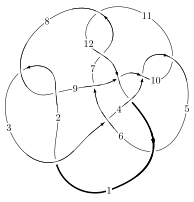
\includegraphics[width=112pt]{../../../GIT/diagram.site/Diagrams/png/2711_12n_0622.png}\\
\ \ \ A knot diagram\footnotemark}&
\allowdisplaybreaks
\textbf{Linearized knot diagam} \\
\cline{2-2}
 &
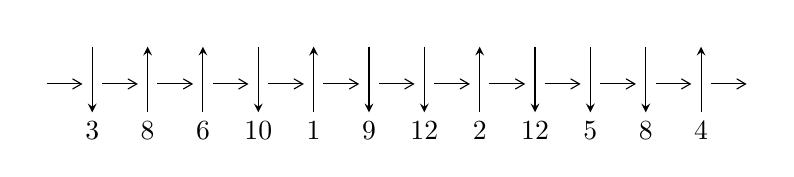
\begin{tikzpicture}[x=20pt, y=17pt]
	% nodes
	\node (C0) at (0, 0) {};
	\node (C1) at (1, 0) {};
	\node (C1U) at (1, +1) {};
	\node (C1D) at (1, -1) {3};

	\node (C2) at (2, 0) {};
	\node (C2U) at (2, +1) {};
	\node (C2D) at (2, -1) {8};

	\node (C3) at (3, 0) {};
	\node (C3U) at (3, +1) {};
	\node (C3D) at (3, -1) {6};

	\node (C4) at (4, 0) {};
	\node (C4U) at (4, +1) {};
	\node (C4D) at (4, -1) {10};

	\node (C5) at (5, 0) {};
	\node (C5U) at (5, +1) {};
	\node (C5D) at (5, -1) {1};

	\node (C6) at (6, 0) {};
	\node (C6U) at (6, +1) {};
	\node (C6D) at (6, -1) {9};

	\node (C7) at (7, 0) {};
	\node (C7U) at (7, +1) {};
	\node (C7D) at (7, -1) {12};

	\node (C8) at (8, 0) {};
	\node (C8U) at (8, +1) {};
	\node (C8D) at (8, -1) {2};

	\node (C9) at (9, 0) {};
	\node (C9U) at (9, +1) {};
	\node (C9D) at (9, -1) {12};

	\node (C10) at (10, 0) {};
	\node (C10U) at (10, +1) {};
	\node (C10D) at (10, -1) {5};

	\node (C11) at (11, 0) {};
	\node (C11U) at (11, +1) {};
	\node (C11D) at (11, -1) {8};

	\node (C12) at (12, 0) {};
	\node (C12U) at (12, +1) {};
	\node (C12D) at (12, -1) {4};
	\node (C13) at (13, 0) {};

	% arrows
	\draw[->,>={angle 60}]
	(C0) edge (C1) (C1) edge (C2) (C2) edge (C3) (C3) edge (C4) (C4) edge (C5) (C5) edge (C6) (C6) edge (C7) (C7) edge (C8) (C8) edge (C9) (C9) edge (C10) (C10) edge (C11) (C11) edge (C12) (C12) edge (C13) ;	\draw[->,>=stealth]
	(C1U) edge (C1D) (C2D) edge (C2U) (C3D) edge (C3U) (C4U) edge (C4D) (C5D) edge (C5U) (C6U) edge (C6D) (C7U) edge (C7D) (C8D) edge (C8U) (C9U) edge (C9D) (C10U) edge (C10D) (C11U) edge (C11D) (C12D) edge (C12U) ;
	\end{tikzpicture} \\
\hhline{~~} \\& 
\textbf{Solving Sequence} \\ \cline{2-2} 
 &
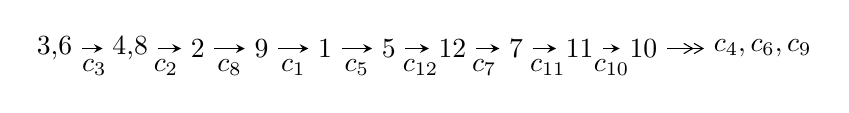
\begin{tikzpicture}[x=23pt, y=7pt]
	% node
	\node (A0) at (-1/8, 0) {3,6};
	\node (A1) at (17/16, 0) {4,8};
	\node (A2) at (17/8, 0) {2};
	\node (A3) at (25/8, 0) {9};
	\node (A4) at (33/8, 0) {1};
	\node (A5) at (41/8, 0) {5};
	\node (A6) at (49/8, 0) {12};
	\node (A7) at (57/8, 0) {7};
	\node (A8) at (65/8, 0) {11};
	\node (A9) at (73/8, 0) {10};
	\node (C1) at (1/2, -1) {$c_{3}$};
	\node (C2) at (13/8, -1) {$c_{2}$};
	\node (C3) at (21/8, -1) {$c_{8}$};
	\node (C4) at (29/8, -1) {$c_{1}$};
	\node (C5) at (37/8, -1) {$c_{5}$};
	\node (C6) at (45/8, -1) {$c_{12}$};
	\node (C7) at (53/8, -1) {$c_{7}$};
	\node (C8) at (61/8, -1) {$c_{11}$};
	\node (C9) at (69/8, -1) {$c_{10}$};
	\node (A10) at (11, 0) {$c_{4},c_{6},c_{9}$};

	% edge
	\draw[->,>=stealth]	
	(A0) edge (A1) (A1) edge (A2) (A2) edge (A3) (A3) edge (A4) (A4) edge (A5) (A5) edge (A6) (A6) edge (A7) (A7) edge (A8) (A8) edge (A9) ;
	\draw[->>,>={angle 60}]	
	(A9) edge (A10);
\end{tikzpicture} \\ 

\end{tabular} \\

\footnotetext{
The image of knot diagram is generated by the software ``\textbf{Draw programme}" developed by Andrew Bartholomew(\url{http://www.layer8.co.uk/maths/draw/index.htm\#Running-draw}), where we modified some parts for our purpose(\url{https://github.com/CATsTAILs/LinksPainter}).
}\phantom \\ \newline 
\centering \textbf{Ideals for irreducible components\footnotemark of $X_{\text{par}}$} 
 
\begin{align*}
I^u_{1}&=\langle 
4.92452\times10^{287} u^{78}+1.93718\times10^{288} u^{77}+\cdots+2.14374\times10^{288} b+4.20946\times10^{287},\\
\phantom{I^u_{1}}&\phantom{= \langle  }1.49187\times10^{288} u^{78}+4.54831\times10^{288} u^{77}+\cdots+2.14374\times10^{288} a+3.02836\times10^{288},\;u^{79}+4 u^{78}+\cdots-15 u-2\rangle \\
I^u_{2}&=\langle 
8.86602\times10^{26} u^{29}+4.96461\times10^{27} u^{28}+\cdots+2.07890\times10^{27} b-8.46568\times10^{27},\\
\phantom{I^u_{2}}&\phantom{= \langle  }-2.14303\times10^{27} u^{29}-1.46624\times10^{28} u^{28}+\cdots+2.07890\times10^{27} a+2.20584\times10^{27},\;u^{30}+7 u^{29}+\cdots-2 u+1\rangle \\
\\
\end{align*}
\raggedright * 2 irreducible components of $\dim_{\mathbb{C}}=0$, with total 109 representations.\\
\footnotetext{All coefficients of polynomials are rational numbers. But the coefficients are sometimes approximated in decimal forms when there is not enough margin.}
\newpage
\renewcommand{\arraystretch}{1}
\centering \section*{I. $I^u_{1}= \langle 4.92\times10^{287} u^{78}+1.94\times10^{288} u^{77}+\cdots+2.14\times10^{288} b+4.21\times10^{287},\;1.49\times10^{288} u^{78}+4.55\times10^{288} u^{77}+\cdots+2.14\times10^{288} a+3.03\times10^{288},\;u^{79}+4 u^{78}+\cdots-15 u-2 \rangle$}
\flushleft \textbf{(i) Arc colorings}\\
\begin{tabular}{m{7pt} m{180pt} m{7pt} m{180pt} }
\flushright $a_{3}=$&$\begin{pmatrix}1\\0\end{pmatrix}$ \\
\flushright $a_{6}=$&$\begin{pmatrix}0\\u\end{pmatrix}$ \\
\flushright $a_{4}=$&$\begin{pmatrix}1\\- u^2\end{pmatrix}$ \\
\flushright $a_{8}=$&$\begin{pmatrix}-0.695917 u^{78}-2.12167 u^{77}+\cdots+3.19841 u-1.41265\\-0.229716 u^{78}-0.903642 u^{77}+\cdots+3.41853 u-0.196360\end{pmatrix}$ \\
\flushright $a_{2}=$&$\begin{pmatrix}-1.80728 u^{78}-6.63665 u^{77}+\cdots+33.4230 u+4.46023\\0.282833 u^{78}+0.998771 u^{77}+\cdots+5.24866 u+1.63785\end{pmatrix}$ \\
\flushright $a_{9}=$&$\begin{pmatrix}-1.28126 u^{78}-4.73105 u^{77}+\cdots+59.6882 u+8.86459\\-0.0732110 u^{78}-0.146482 u^{77}+\cdots-14.5367 u-3.50294\end{pmatrix}$ \\
\flushright $a_{1}=$&$\begin{pmatrix}-1.52445 u^{78}-5.63788 u^{77}+\cdots+38.6717 u+6.09808\\0.282833 u^{78}+0.998771 u^{77}+\cdots+5.24866 u+1.63785\end{pmatrix}$ \\
\flushright $a_{5}=$&$\begin{pmatrix}-0.671308 u^{78}-3.15509 u^{77}+\cdots+49.0749 u+14.1783\\0.212306 u^{78}+0.790438 u^{77}+\cdots-8.06833 u-1.68927\end{pmatrix}$ \\
\flushright $a_{12}=$&$\begin{pmatrix}-1.73942 u^{78}-6.33735 u^{77}+\cdots+29.5732 u+3.54039\\0.312581 u^{78}+1.11717 u^{77}+\cdots+3.27223 u+1.31700\end{pmatrix}$ \\
\flushright $a_{7}=$&$\begin{pmatrix}-3.40969 u^{78}-12.5097 u^{77}+\cdots+117.027 u+16.8820\\-0.193655 u^{78}-0.656440 u^{77}+\cdots-7.35796 u-2.70038\end{pmatrix}$ \\
\flushright $a_{11}=$&$\begin{pmatrix}0.593823 u^{78}+1.60440 u^{77}+\cdots+10.7553 u+9.93213\\0.224564 u^{78}+0.848409 u^{77}+\cdots-5.84297 u-1.44066\end{pmatrix}$ \\
\flushright $a_{10}=$&$\begin{pmatrix}1.06875 u^{78}+4.43417 u^{77}+\cdots-57.8967 u-11.3128\\-0.200371 u^{78}-0.773026 u^{77}+\cdots+6.71504 u+0.666681\end{pmatrix}$\\&\end{tabular}
\flushleft \textbf{(ii) Obstruction class $= -1$}\\~\\
\flushleft \textbf{(iii) Cusp Shapes $= -0.466124 u^{78}-1.35878 u^{77}+\cdots-90.0451 u-15.6671$}\\~\\
\newpage\renewcommand{\arraystretch}{1}
\flushleft \textbf{(iv) u-Polynomials at the component}\newline \\
\begin{tabular}{m{50pt}|m{274pt}}
Crossings & \hspace{64pt}u-Polynomials at each crossing \\
\hline $$\begin{aligned}c_{1}\end{aligned}$$&$\begin{aligned}
&u^{79}+43 u^{78}+\cdots-1004 u-100
\end{aligned}$\\
\hline $$\begin{aligned}c_{2},c_{8}\end{aligned}$$&$\begin{aligned}
&u^{79}+3 u^{78}+\cdots-14 u-10
\end{aligned}$\\
\hline $$\begin{aligned}c_{3}\end{aligned}$$&$\begin{aligned}
&u^{79}+4 u^{78}+\cdots-15 u-2
\end{aligned}$\\
\hline $$\begin{aligned}c_{4},c_{10}\end{aligned}$$&$\begin{aligned}
&u^{79}-2 u^{78}+\cdots-120 u+26
\end{aligned}$\\
\hline $$\begin{aligned}c_{5}\end{aligned}$$&$\begin{aligned}
&u^{79}-2 u^{78}+\cdots-8478 u-3078
\end{aligned}$\\
\hline $$\begin{aligned}c_{6}\end{aligned}$$&$\begin{aligned}
&u^{79}-6 u^{78}+\cdots+1496873 u+115748
\end{aligned}$\\
\hline $$\begin{aligned}c_{7},c_{11}\end{aligned}$$&$\begin{aligned}
&u^{79}+4 u^{78}+\cdots+1193295 u-523514
\end{aligned}$\\
\hline $$\begin{aligned}c_{9}\end{aligned}$$&$\begin{aligned}
&u^{79}-5 u^{78}+\cdots+16594 u-12214
\end{aligned}$\\
\hline $$\begin{aligned}c_{12}\end{aligned}$$&$\begin{aligned}
&u^{79}+6 u^{78}+\cdots+45561 u-4572
\end{aligned}$\\
\hline
\end{tabular}\\~\\
\newpage\renewcommand{\arraystretch}{1}
\flushleft \textbf{(v) Riley Polynomials at the component}\newline \\
\begin{tabular}{m{50pt}|m{274pt}}
Crossings & \hspace{64pt}Riley Polynomials at each crossing \\
\hline $$\begin{aligned}c_{1}\end{aligned}$$&$\begin{aligned}
&y^{79}- y^{78}+\cdots+465616 y-10000
\end{aligned}$\\
\hline $$\begin{aligned}c_{2},c_{8}\end{aligned}$$&$\begin{aligned}
&y^{79}+43 y^{78}+\cdots-1004 y-100
\end{aligned}$\\
\hline $$\begin{aligned}c_{3}\end{aligned}$$&$\begin{aligned}
&y^{79}-8 y^{78}+\cdots-151 y-4
\end{aligned}$\\
\hline $$\begin{aligned}c_{4},c_{10}\end{aligned}$$&$\begin{aligned}
&y^{79}-60 y^{78}+\cdots+42480 y-676
\end{aligned}$\\
\hline $$\begin{aligned}c_{5}\end{aligned}$$&$\begin{aligned}
&y^{79}+8 y^{78}+\cdots-207913716 y-9474084
\end{aligned}$\\
\hline $$\begin{aligned}c_{6}\end{aligned}$$&$\begin{aligned}
&y^{79}-116 y^{78}+\cdots+1057720100009 y-13397599504
\end{aligned}$\\
\hline $$\begin{aligned}c_{7},c_{11}\end{aligned}$$&$\begin{aligned}
&y^{79}-90 y^{78}+\cdots+5429126130809 y-274066908196
\end{aligned}$\\
\hline $$\begin{aligned}c_{9}\end{aligned}$$&$\begin{aligned}
&y^{79}-103 y^{78}+\cdots+453343244 y-149181796
\end{aligned}$\\
\hline $$\begin{aligned}c_{12}\end{aligned}$$&$\begin{aligned}
&y^{79}+28 y^{78}+\cdots+771038217 y-20903184
\end{aligned}$\\
\hline
\end{tabular}\\~\\
\newpage\flushleft \textbf{(vi) Complex Volumes and Cusp Shapes}
$$\begin{array}{c|c|c}  
\text{Solutions to }I^u_{1}& \I (\text{vol} + \sqrt{-1}CS) & \text{Cusp shape}\\
 \hline 
\begin{aligned}
u &= \phantom{-}0.816172 + 0.646013 I \\
a &= -1.209900 - 0.076500 I \\
b &= \phantom{-}0.70666 + 1.38162 I\end{aligned}
 & -9.03674 + 7.36246 I & \phantom{-0.000000 } 0 \\ \hline\begin{aligned}
u &= \phantom{-}0.816172 - 0.646013 I \\
a &= -1.209900 + 0.076500 I \\
b &= \phantom{-}0.70666 - 1.38162 I\end{aligned}
 & -9.03674 - 7.36246 I & \phantom{-0.000000 } 0 \\ \hline\begin{aligned}
u &= -0.851565 + 0.604278 I \\
a &= -0.096173 + 0.355509 I \\
b &= -0.432323 - 0.206165 I\end{aligned}
 & -0.59266 - 4.94262 I & \phantom{-0.000000 } 0 \\ \hline\begin{aligned}
u &= -0.851565 - 0.604278 I \\
a &= -0.096173 - 0.355509 I \\
b &= -0.432323 + 0.206165 I\end{aligned}
 & -0.59266 + 4.94262 I & \phantom{-0.000000 } 0 \\ \hline\begin{aligned}
u &= -1.034490 + 0.191822 I \\
a &= -0.361792 - 0.581823 I \\
b &= -0.241504 + 0.613860 I\end{aligned}
 & -0.96739 - 5.14315 I & \phantom{-0.000000 } 0 \\ \hline\begin{aligned}
u &= -1.034490 - 0.191822 I \\
a &= -0.361792 + 0.581823 I \\
b &= -0.241504 - 0.613860 I\end{aligned}
 & -0.96739 + 5.14315 I & \phantom{-0.000000 } 0 \\ \hline\begin{aligned}
u &= \phantom{-}0.013775 + 0.937830 I \\
a &= \phantom{-}0.51318 + 1.52869 I \\
b &= \phantom{-}0.585484 + 0.360436 I\end{aligned}
 & -8.21660 + 2.04904 I & -8.02716 - 3.74321 I \\ \hline\begin{aligned}
u &= \phantom{-}0.013775 - 0.937830 I \\
a &= \phantom{-}0.51318 - 1.52869 I \\
b &= \phantom{-}0.585484 - 0.360436 I\end{aligned}
 & -8.21660 - 2.04904 I & -8.02716 + 3.74321 I \\ \hline\begin{aligned}
u &= \phantom{-}0.700344 + 0.855508 I \\
a &= -0.934162 + 0.922785 I \\
b &= \phantom{-}0.369105 + 1.037020 I\end{aligned}
 & -1.01865 + 3.56912 I & \phantom{-0.000000 } 0 \\ \hline\begin{aligned}
u &= \phantom{-}0.700344 - 0.855508 I \\
a &= -0.934162 - 0.922785 I \\
b &= \phantom{-}0.369105 - 1.037020 I\end{aligned}
 & -1.01865 - 3.56912 I & \phantom{-0.000000 } 0\\
 \hline 
 \end{array}$$\newpage$$\begin{array}{c|c|c}  
\text{Solutions to }I^u_{1}& \I (\text{vol} + \sqrt{-1}CS) & \text{Cusp shape}\\
 \hline 
\begin{aligned}
u &= \phantom{-}0.448324 + 1.013580 I \\
a &= \phantom{-}0.752506 - 0.152892 I \\
b &= \phantom{-}0.520524 - 1.124140 I\end{aligned}
 & -10.49970 - 2.46799 I & \phantom{-0.000000 } 0 \\ \hline\begin{aligned}
u &= \phantom{-}0.448324 - 1.013580 I \\
a &= \phantom{-}0.752506 + 0.152892 I \\
b &= \phantom{-}0.520524 + 1.124140 I\end{aligned}
 & -10.49970 + 2.46799 I & \phantom{-0.000000 } 0 \\ \hline\begin{aligned}
u &= -0.633902 + 0.922767 I \\
a &= \phantom{-}1.021790 + 0.912971 I \\
b &= -0.461486 + 1.144140 I\end{aligned}
 & -3.30115 - 8.89430 I & \phantom{-0.000000 } 0 \\ \hline\begin{aligned}
u &= -0.633902 - 0.922767 I \\
a &= \phantom{-}1.021790 - 0.912971 I \\
b &= -0.461486 - 1.144140 I\end{aligned}
 & -3.30115 + 8.89430 I & \phantom{-0.000000 } 0 \\ \hline\begin{aligned}
u &= -0.660179 + 0.559566 I \\
a &= \phantom{-}1.78017 - 0.22112 I \\
b &= -0.578067 + 1.168530 I\end{aligned}
 & -5.07794 - 5.70686 I & -7.10807 - 1.44397 I \\ \hline\begin{aligned}
u &= -0.660179 - 0.559566 I \\
a &= \phantom{-}1.78017 + 0.22112 I \\
b &= -0.578067 - 1.168530 I\end{aligned}
 & -5.07794 + 5.70686 I & -7.10807 + 1.44397 I \\ \hline\begin{aligned}
u &= \phantom{-}1.085140 + 0.338076 I \\
a &= \phantom{-}0.255368 + 1.163830 I \\
b &= \phantom{-}0.070726 - 0.734940 I\end{aligned}
 & \phantom{-}0.773012 + 1.152010 I & \phantom{-0.000000 } 0 \\ \hline\begin{aligned}
u &= \phantom{-}1.085140 - 0.338076 I \\
a &= \phantom{-}0.255368 - 1.163830 I \\
b &= \phantom{-}0.070726 + 0.734940 I\end{aligned}
 & \phantom{-}0.773012 - 1.152010 I & \phantom{-0.000000 } 0 \\ \hline\begin{aligned}
u &= -0.937083 + 0.647339 I \\
a &= -1.101110 + 0.038652 I \\
b &= \phantom{-}0.744421 - 0.366284 I\end{aligned}
 & -0.58487 - 4.01785 I & \phantom{-0.000000 } 0 \\ \hline\begin{aligned}
u &= -0.937083 - 0.647339 I \\
a &= -1.101110 - 0.038652 I \\
b &= \phantom{-}0.744421 + 0.366284 I\end{aligned}
 & -0.58487 + 4.01785 I & \phantom{-0.000000 } 0\\
 \hline 
 \end{array}$$\newpage$$\begin{array}{c|c|c}  
\text{Solutions to }I^u_{1}& \I (\text{vol} + \sqrt{-1}CS) & \text{Cusp shape}\\
 \hline 
\begin{aligned}
u &= -0.220511 + 1.146240 I \\
a &= -0.436797 - 0.196503 I \\
b &= -0.295511 - 1.078110 I\end{aligned}
 & -7.37626 + 2.11501 I & \phantom{-0.000000 } 0 \\ \hline\begin{aligned}
u &= -0.220511 - 1.146240 I \\
a &= -0.436797 + 0.196503 I \\
b &= -0.295511 + 1.078110 I\end{aligned}
 & -7.37626 - 2.11501 I & \phantom{-0.000000 } 0 \\ \hline\begin{aligned}
u &= -0.868469 + 0.803966 I \\
a &= -0.675181 - 0.843567 I \\
b &= \phantom{-}0.772773 + 0.559676 I\end{aligned}
 & -0.96281 - 1.45120 I & \phantom{-0.000000 } 0 \\ \hline\begin{aligned}
u &= -0.868469 - 0.803966 I \\
a &= -0.675181 + 0.843567 I \\
b &= \phantom{-}0.772773 - 0.559676 I\end{aligned}
 & -0.96281 + 1.45120 I & \phantom{-0.000000 } 0 \\ \hline\begin{aligned}
u &= -0.574732 + 1.037720 I \\
a &= \phantom{-}0.152511 + 0.119525 I \\
b &= -0.15417 - 1.51805 I\end{aligned}
 & -15.5511 - 5.8296 I & \phantom{-0.000000 } 0 \\ \hline\begin{aligned}
u &= -0.574732 - 1.037720 I \\
a &= \phantom{-}0.152511 - 0.119525 I \\
b &= -0.15417 + 1.51805 I\end{aligned}
 & -15.5511 + 5.8296 I & \phantom{-0.000000 } 0 \\ \hline\begin{aligned}
u &= \phantom{-}0.779928 + 0.219709 I \\
a &= -0.0845212 + 0.0646654 I \\
b &= \phantom{-}0.448745 + 0.043523 I\end{aligned}
 & \phantom{-}1.49146 + 0.64236 I & \phantom{-}4.77435 + 0.42718 I \\ \hline\begin{aligned}
u &= \phantom{-}0.779928 - 0.219709 I \\
a &= -0.0845212 - 0.0646654 I \\
b &= \phantom{-}0.448745 - 0.043523 I\end{aligned}
 & \phantom{-}1.49146 - 0.64236 I & \phantom{-}4.77435 - 0.42718 I \\ \hline\begin{aligned}
u &= -0.069592 + 1.215010 I \\
a &= -0.284409 + 1.131300 I \\
b &= -0.153291 + 0.859355 I\end{aligned}
 & -6.20670 + 0.35244 I & \phantom{-0.000000 } 0 \\ \hline\begin{aligned}
u &= -0.069592 - 1.215010 I \\
a &= -0.284409 - 1.131300 I \\
b &= -0.153291 - 0.859355 I\end{aligned}
 & -6.20670 - 0.35244 I & \phantom{-0.000000 } 0\\
 \hline 
 \end{array}$$\newpage$$\begin{array}{c|c|c}  
\text{Solutions to }I^u_{1}& \I (\text{vol} + \sqrt{-1}CS) & \text{Cusp shape}\\
 \hline 
\begin{aligned}
u &= -0.381706 + 0.616663 I \\
a &= -0.646954 - 0.302471 I \\
b &= \phantom{-}0.63548 + 1.31769 I\end{aligned}
 & -3.12841 + 1.60812 I & -9.18560 + 2.80861 I \\ \hline\begin{aligned}
u &= -0.381706 - 0.616663 I \\
a &= -0.646954 + 0.302471 I \\
b &= \phantom{-}0.63548 - 1.31769 I\end{aligned}
 & -3.12841 - 1.60812 I & -9.18560 - 2.80861 I \\ \hline\begin{aligned}
u &= -0.588655 + 1.137800 I \\
a &= \phantom{-}0.137393 + 0.569291 I \\
b &= \phantom{-}0.046183 + 1.104620 I\end{aligned}
 & -6.54145 - 0.12000 I & \phantom{-0.000000 } 0 \\ \hline\begin{aligned}
u &= -0.588655 - 1.137800 I \\
a &= \phantom{-}0.137393 - 0.569291 I \\
b &= \phantom{-}0.046183 - 1.104620 I\end{aligned}
 & -6.54145 + 0.12000 I & \phantom{-0.000000 } 0 \\ \hline\begin{aligned}
u &= -0.926132 + 0.904026 I \\
a &= -1.89386 - 0.43776 I \\
b &= \phantom{-}0.663678 - 1.048350 I\end{aligned}
 & -2.40423 - 6.89015 I & \phantom{-0.000000 } 0 \\ \hline\begin{aligned}
u &= -0.926132 - 0.904026 I \\
a &= -1.89386 + 0.43776 I \\
b &= \phantom{-}0.663678 + 1.048350 I\end{aligned}
 & -2.40423 + 6.89015 I & \phantom{-0.000000 } 0 \\ \hline\begin{aligned}
u &= \phantom{-}0.043690 + 0.643510 I \\
a &= \phantom{-}1.38661 - 1.02506 I \\
b &= -0.652287 - 0.993200 I\end{aligned}
 & -2.52587 + 5.75002 I & -4.75156 - 7.12777 I \\ \hline\begin{aligned}
u &= \phantom{-}0.043690 - 0.643510 I \\
a &= \phantom{-}1.38661 + 1.02506 I \\
b &= -0.652287 + 0.993200 I\end{aligned}
 & -2.52587 - 5.75002 I & -4.75156 + 7.12777 I \\ \hline\begin{aligned}
u &= \phantom{-}0.630240\phantom{ +0.000000I} \\
a &= -1.27668\phantom{ +0.000000I} \\
b &= \phantom{-}1.47192\phantom{ +0.000000I}\end{aligned}
 & -5.02482\phantom{ +0.000000I} & \phantom{-}5.52250\phantom{ +0.000000I} \\ \hline\begin{aligned}
u &= -0.328954 + 0.535707 I \\
a &= \phantom{-}0.704767 + 0.026780 I \\
b &= -0.568775 + 0.504540 I\end{aligned}
 & -1.47696 + 0.84526 I & -4.04601 - 1.22760 I\\
 \hline 
 \end{array}$$\newpage$$\begin{array}{c|c|c}  
\text{Solutions to }I^u_{1}& \I (\text{vol} + \sqrt{-1}CS) & \text{Cusp shape}\\
 \hline 
\begin{aligned}
u &= -0.328954 - 0.535707 I \\
a &= \phantom{-}0.704767 - 0.026780 I \\
b &= -0.568775 - 0.504540 I\end{aligned}
 & -1.47696 - 0.84526 I & -4.04601 + 1.22760 I \\ \hline\begin{aligned}
u &= -0.948643 + 1.013220 I \\
a &= \phantom{-}1.25177 + 0.68906 I \\
b &= -0.720763 + 0.189367 I\end{aligned}
 & -8.97766 + 3.13474 I & \phantom{-0.000000 } 0 \\ \hline\begin{aligned}
u &= -0.948643 - 1.013220 I \\
a &= \phantom{-}1.25177 - 0.68906 I \\
b &= -0.720763 - 0.189367 I\end{aligned}
 & -8.97766 - 3.13474 I & \phantom{-0.000000 } 0 \\ \hline\begin{aligned}
u &= \phantom{-}0.089016 + 0.565790 I \\
a &= \phantom{-}0.924897 + 0.743590 I \\
b &= -0.094656 + 0.871815 I\end{aligned}
 & -1.11180 + 1.12663 I & -4.25436 - 4.77232 I \\ \hline\begin{aligned}
u &= \phantom{-}0.089016 - 0.565790 I \\
a &= \phantom{-}0.924897 - 0.743590 I \\
b &= -0.094656 - 0.871815 I\end{aligned}
 & -1.11180 - 1.12663 I & -4.25436 + 4.77232 I \\ \hline\begin{aligned}
u &= -1.01144 + 1.00979 I \\
a &= \phantom{-}1.026240 + 0.432846 I \\
b &= -1.103030 - 0.337146 I\end{aligned}
 & -8.88395 - 10.49540 I & \phantom{-0.000000 } 0 \\ \hline\begin{aligned}
u &= -1.01144 - 1.00979 I \\
a &= \phantom{-}1.026240 - 0.432846 I \\
b &= -1.103030 + 0.337146 I\end{aligned}
 & -8.88395 + 10.49540 I & \phantom{-0.000000 } 0 \\ \hline\begin{aligned}
u &= \phantom{-}1.14947 + 0.85016 I \\
a &= \phantom{-}0.669035 - 0.352609 I \\
b &= -0.724647 + 0.698496 I\end{aligned}
 & \phantom{-}3.57978 + 1.16112 I & \phantom{-0.000000 } 0 \\ \hline\begin{aligned}
u &= \phantom{-}1.14947 - 0.85016 I \\
a &= \phantom{-}0.669035 + 0.352609 I \\
b &= -0.724647 - 0.698496 I\end{aligned}
 & \phantom{-}3.57978 - 1.16112 I & \phantom{-0.000000 } 0 \\ \hline\begin{aligned}
u &= \phantom{-}0.414725 + 0.345278 I \\
a &= -4.97629 - 2.25758 I \\
b &= \phantom{-}0.417806 + 1.104800 I\end{aligned}
 & -11.26510 + 5.06614 I & -9.4830 - 11.2407 I\\
 \hline 
 \end{array}$$\newpage$$\begin{array}{c|c|c}  
\text{Solutions to }I^u_{1}& \I (\text{vol} + \sqrt{-1}CS) & \text{Cusp shape}\\
 \hline 
\begin{aligned}
u &= \phantom{-}0.414725 - 0.345278 I \\
a &= -4.97629 + 2.25758 I \\
b &= \phantom{-}0.417806 - 1.104800 I\end{aligned}
 & -11.26510 - 5.06614 I & -9.4830 + 11.2407 I \\ \hline\begin{aligned}
u &= \phantom{-}1.04842 + 1.01862 I \\
a &= -1.203070 + 0.380286 I \\
b &= \phantom{-}0.871333 - 0.297517 I\end{aligned}
 & -3.99736 + 3.71610 I & \phantom{-0.000000 } 0 \\ \hline\begin{aligned}
u &= \phantom{-}1.04842 - 1.01862 I \\
a &= -1.203070 - 0.380286 I \\
b &= \phantom{-}0.871333 + 0.297517 I\end{aligned}
 & -3.99736 - 3.71610 I & \phantom{-0.000000 } 0 \\ \hline\begin{aligned}
u &= \phantom{-}0.99411 + 1.13893 I \\
a &= \phantom{-}1.265690 - 0.370176 I \\
b &= -0.682775 - 1.000360 I\end{aligned}
 & \phantom{-}2.66017 + 6.57787 I & \phantom{-0.000000 } 0 \\ \hline\begin{aligned}
u &= \phantom{-}0.99411 - 1.13893 I \\
a &= \phantom{-}1.265690 + 0.370176 I \\
b &= -0.682775 + 1.000360 I\end{aligned}
 & \phantom{-}2.66017 - 6.57787 I & \phantom{-0.000000 } 0 \\ \hline\begin{aligned}
u &= -0.313888 + 0.338273 I \\
a &= -2.50850 - 0.01377 I \\
b &= \phantom{-}0.528219 - 0.898276 I\end{aligned}
 & -0.20481 - 2.07908 I & -2.26565 + 3.54284 I \\ \hline\begin{aligned}
u &= -0.313888 - 0.338273 I \\
a &= -2.50850 + 0.01377 I \\
b &= \phantom{-}0.528219 + 0.898276 I\end{aligned}
 & -0.20481 + 2.07908 I & -2.26565 - 3.54284 I \\ \hline\begin{aligned}
u &= -1.23948 + 0.96164 I \\
a &= -1.160200 - 0.083777 I \\
b &= \phantom{-}0.387636 - 1.191240 I\end{aligned}
 & -4.64705 - 7.48016 I & \phantom{-0.000000 } 0 \\ \hline\begin{aligned}
u &= -1.23948 - 0.96164 I \\
a &= -1.160200 + 0.083777 I \\
b &= \phantom{-}0.387636 + 1.191240 I\end{aligned}
 & -4.64705 + 7.48016 I & \phantom{-0.000000 } 0 \\ \hline\begin{aligned}
u &= -1.45045 + 0.60559 I \\
a &= \phantom{-}1.51675 - 0.63151 I \\
b &= -0.404021 + 1.183230 I\end{aligned}
 & -12.70520 - 0.62704 I & \phantom{-0.000000 } 0\\
 \hline 
 \end{array}$$\newpage$$\begin{array}{c|c|c}  
\text{Solutions to }I^u_{1}& \I (\text{vol} + \sqrt{-1}CS) & \text{Cusp shape}\\
 \hline 
\begin{aligned}
u &= -1.45045 - 0.60559 I \\
a &= \phantom{-}1.51675 + 0.63151 I \\
b &= -0.404021 - 1.183230 I\end{aligned}
 & -12.70520 + 0.62704 I & \phantom{-0.000000 } 0 \\ \hline\begin{aligned}
u &= -1.14535 + 1.15657 I \\
a &= \phantom{-}1.43220 + 0.07872 I \\
b &= -0.67392 + 1.25371 I\end{aligned}
 & -11.7549 - 16.8301 I & \phantom{-0.000000 } 0 \\ \hline\begin{aligned}
u &= -1.14535 - 1.15657 I \\
a &= \phantom{-}1.43220 - 0.07872 I \\
b &= -0.67392 - 1.25371 I\end{aligned}
 & -11.7549 + 16.8301 I & \phantom{-0.000000 } 0 \\ \hline\begin{aligned}
u &= -0.273434 + 0.201008 I \\
a &= \phantom{-}7.60180 + 6.40532 I \\
b &= \phantom{-}0.152256 - 0.562228 I\end{aligned}
 & -9.01819 + 2.00460 I & -0.76875 - 9.29624 I \\ \hline\begin{aligned}
u &= -0.273434 - 0.201008 I \\
a &= \phantom{-}7.60180 - 6.40532 I \\
b &= \phantom{-}0.152256 + 0.562228 I\end{aligned}
 & -9.01819 - 2.00460 I & -0.76875 + 9.29624 I \\ \hline\begin{aligned}
u &= \phantom{-}0.66920 + 1.56410 I \\
a &= -0.404676 + 0.100855 I \\
b &= \phantom{-}0.286627 - 1.202720 I\end{aligned}
 & -8.81807 + 0.31313 I & \phantom{-0.000000 } 0 \\ \hline\begin{aligned}
u &= \phantom{-}0.66920 - 1.56410 I \\
a &= -0.404676 - 0.100855 I \\
b &= \phantom{-}0.286627 + 1.202720 I\end{aligned}
 & -8.81807 - 0.31313 I & \phantom{-0.000000 } 0 \\ \hline\begin{aligned}
u &= -0.118942 + 0.240216 I \\
a &= \phantom{-}2.08281 + 1.06752 I \\
b &= -1.091290 - 0.434988 I\end{aligned}
 & -2.41782 - 0.14514 I & -1.32526 - 13.85499 I \\ \hline\begin{aligned}
u &= -0.118942 - 0.240216 I \\
a &= \phantom{-}2.08281 - 1.06752 I \\
b &= -1.091290 + 0.434988 I\end{aligned}
 & -2.41782 + 0.14514 I & -1.32526 + 13.85499 I \\ \hline\begin{aligned}
u &= \phantom{-}0.121981 + 0.177501 I \\
a &= \phantom{-}2.08700 - 0.27369 I \\
b &= -0.60868 - 1.42128 I\end{aligned}
 & -2.62990 - 0.59843 I & -17.8564 - 15.9399 I\\
 \hline 
 \end{array}$$\newpage$$\begin{array}{c|c|c}  
\text{Solutions to }I^u_{1}& \I (\text{vol} + \sqrt{-1}CS) & \text{Cusp shape}\\
 \hline 
\begin{aligned}
u &= \phantom{-}0.121981 - 0.177501 I \\
a &= \phantom{-}2.08700 + 0.27369 I \\
b &= -0.60868 + 1.42128 I\end{aligned}
 & -2.62990 + 0.59843 I & -17.8564 + 15.9399 I \\ \hline\begin{aligned}
u &= \phantom{-}1.78645 + 0.03549 I \\
a &= \phantom{-}1.351430 + 0.373710 I \\
b &= -0.605004 - 0.852194 I\end{aligned}
 & \phantom{-}4.83036 + 2.38662 I & \phantom{-0.000000 } 0 \\ \hline\begin{aligned}
u &= \phantom{-}1.78645 - 0.03549 I \\
a &= \phantom{-}1.351430 - 0.373710 I \\
b &= -0.605004 + 0.852194 I\end{aligned}
 & \phantom{-}4.83036 - 2.38662 I & \phantom{-0.000000 } 0 \\ \hline\begin{aligned}
u &= \phantom{-}1.38258 + 1.16195 I \\
a &= -1.381930 - 0.144564 I \\
b &= \phantom{-}0.583135 + 1.190080 I\end{aligned}
 & -6.70689 + 9.09405 I & \phantom{-0.000000 } 0 \\ \hline\begin{aligned}
u &= \phantom{-}1.38258 - 1.16195 I \\
a &= -1.381930 + 0.144564 I \\
b &= \phantom{-}0.583135 - 1.190080 I\end{aligned}
 & -6.70689 - 9.09405 I & \phantom{-0.000000 } 0 \\ \hline\begin{aligned}
u &= -1.22703 + 1.33810 I \\
a &= \phantom{-}0.465359 + 0.291972 I \\
b &= -0.520857 - 1.179320 I\end{aligned}
 & -11.8473 + 7.8938 I & \phantom{-0.000000 } 0 \\ \hline\begin{aligned}
u &= -1.22703 - 1.33810 I \\
a &= \phantom{-}0.465359 - 0.291972 I \\
b &= -0.520857 + 1.179320 I\end{aligned}
 & -11.8473 - 7.8938 I & \phantom{-0.000000 } 0 \\ \hline\begin{aligned}
u &= \phantom{-}1.94618 + 0.21387 I \\
a &= \phantom{-}0.868595 + 0.099321 I \\
b &= -0.259693 - 0.876278 I\end{aligned}
 & \phantom{-}2.80268 + 1.18375 I & \phantom{-0.000000 } 0 \\ \hline\begin{aligned}
u &= \phantom{-}1.94618 - 0.21387 I \\
a &= \phantom{-}0.868595 - 0.099321 I \\
b &= -0.259693 + 0.876278 I\end{aligned}
 & \phantom{-}2.80268 - 1.18375 I & \phantom{-0.000000 } 0\\
 \hline 
 \end{array}$$\newpage\newpage\renewcommand{\arraystretch}{1}
\centering \section*{II. $I^u_{2}= \langle 8.87\times10^{26} u^{29}+4.96\times10^{27} u^{28}+\cdots+2.08\times10^{27} b-8.47\times10^{27},\;-2.14\times10^{27} u^{29}-1.47\times10^{28} u^{28}+\cdots+2.08\times10^{27} a+2.21\times10^{27},\;u^{30}+7 u^{29}+\cdots-2 u+1 \rangle$}
\flushleft \textbf{(i) Arc colorings}\\
\begin{tabular}{m{7pt} m{180pt} m{7pt} m{180pt} }
\flushright $a_{3}=$&$\begin{pmatrix}1\\0\end{pmatrix}$ \\
\flushright $a_{6}=$&$\begin{pmatrix}0\\u\end{pmatrix}$ \\
\flushright $a_{4}=$&$\begin{pmatrix}1\\- u^2\end{pmatrix}$ \\
\flushright $a_{8}=$&$\begin{pmatrix}1.03085 u^{29}+7.05295 u^{28}+\cdots+12.2937 u-1.06106\\-0.426476 u^{29}-2.38809 u^{28}+\cdots-10.2361 u+4.07219\end{pmatrix}$ \\
\flushright $a_{2}=$&$\begin{pmatrix}-1.29736 u^{29}-8.81885 u^{28}+\cdots-17.3636 u+4.06889\\2.19676 u^{29}+14.7075 u^{28}+\cdots+28.4474 u-7.43484\end{pmatrix}$ \\
\flushright $a_{9}=$&$\begin{pmatrix}0.652770 u^{29}+4.35608 u^{28}+\cdots+14.2719 u-2.77345\\-1.82323 u^{29}-12.2133 u^{28}+\cdots-29.2448 u+6.44625\end{pmatrix}$ \\
\flushright $a_{1}=$&$\begin{pmatrix}0.899401 u^{29}+5.88861 u^{28}+\cdots+11.0838 u-3.36596\\2.19676 u^{29}+14.7075 u^{28}+\cdots+28.4474 u-7.43484\end{pmatrix}$ \\
\flushright $a_{5}=$&$\begin{pmatrix}-0.103982 u^{29}-0.503391 u^{28}+\cdots-3.73912 u+0.326999\\-0.631706 u^{29}-4.65881 u^{28}+\cdots-1.99763 u-0.427052\end{pmatrix}$ \\
\flushright $a_{12}=$&$\begin{pmatrix}-1.11318 u^{29}-7.51504 u^{28}+\cdots-15.6498 u+3.66170\\1.91296 u^{29}+12.7681 u^{28}+\cdots+25.0660 u-6.75043\end{pmatrix}$ \\
\flushright $a_{7}=$&$\begin{pmatrix}0.584554 u^{29}+3.97113 u^{28}+\cdots+14.7136 u-2.86263\\-1.71193 u^{29}-11.4621 u^{28}+\cdots-26.7669 u+6.11442\end{pmatrix}$ \\
\flushright $a_{11}=$&$\begin{pmatrix}0.115312 u^{29}+0.750103 u^{28}+\cdots+0.568560 u+1.49311\\-0.197879 u^{29}-1.48329 u^{28}+\cdots-1.29316 u-1.23882\end{pmatrix}$ \\
\flushright $a_{10}=$&$\begin{pmatrix}0.804684 u^{29}+5.84280 u^{28}+\cdots+4.74884 u+1.14498\\0.204268 u^{29}+1.47370 u^{28}+\cdots+0.799106 u+0.163661\end{pmatrix}$\\&\end{tabular}
\flushleft \textbf{(ii) Obstruction class $= 1$}\\~\\
\flushleft \textbf{(iii) Cusp Shapes $= -\frac{16094927794191462172380835339}{1039451181930225503654703338} u^{29}-\frac{57469821610208664971093176195}{519725590965112751827351669} u^{28}+\cdots-\frac{62817133116220172602979033368}{519725590965112751827351669} u-\frac{17691556347968942647146425724}{519725590965112751827351669}$}\\~\\
\newpage\renewcommand{\arraystretch}{1}
\flushleft \textbf{(iv) u-Polynomials at the component}\newline \\
\begin{tabular}{m{50pt}|m{274pt}}
Crossings & \hspace{64pt}u-Polynomials at each crossing \\
\hline $$\begin{aligned}c_{1}\end{aligned}$$&$\begin{aligned}
&u^{30}-16 u^{29}+\cdots-68 u+4
\end{aligned}$\\
\hline $$\begin{aligned}c_{2}\end{aligned}$$&$\begin{aligned}
&u^{30}+2 u^{29}+\cdots+17 u^2+2
\end{aligned}$\\
\hline $$\begin{aligned}c_{3}\end{aligned}$$&$\begin{aligned}
&u^{30}+7 u^{29}+\cdots-2 u+1
\end{aligned}$\\
\hline $$\begin{aligned}c_{4}\end{aligned}$$&$\begin{aligned}
&u^{30}- u^{29}+\cdots-2 u+2
\end{aligned}$\\
\hline $$\begin{aligned}c_{5}\end{aligned}$$&$\begin{aligned}
&u^{30}+u^{29}+\cdots-10 u+2
\end{aligned}$\\
\hline $$\begin{aligned}c_{6}\end{aligned}$$&$\begin{aligned}
&u^{30}-7 u^{29}+\cdots-381 u+29
\end{aligned}$\\
\hline $$\begin{aligned}c_{7}\end{aligned}$$&$\begin{aligned}
&u^{30}- u^{29}+\cdots-2 u+1
\end{aligned}$\\
\hline $$\begin{aligned}c_{8}\end{aligned}$$&$\begin{aligned}
&u^{30}-2 u^{29}+\cdots+17 u^2+2
\end{aligned}$\\
\hline $$\begin{aligned}c_{9}\end{aligned}$$&$\begin{aligned}
&u^{30}-14 u^{29}+\cdots-394 u+34
\end{aligned}$\\
\hline $$\begin{aligned}c_{10}\end{aligned}$$&$\begin{aligned}
&u^{30}+u^{29}+\cdots+2 u+2
\end{aligned}$\\
\hline $$\begin{aligned}c_{11}\end{aligned}$$&$\begin{aligned}
&u^{30}+u^{29}+\cdots+2 u+1
\end{aligned}$\\
\hline $$\begin{aligned}c_{12}\end{aligned}$$&$\begin{aligned}
&u^{30}- u^{29}+\cdots- u+1
\end{aligned}$\\
\hline
\end{tabular}\\~\\
\newpage\renewcommand{\arraystretch}{1}
\flushleft \textbf{(v) Riley Polynomials at the component}\newline \\
\begin{tabular}{m{50pt}|m{274pt}}
Crossings & \hspace{64pt}Riley Polynomials at each crossing \\
\hline $$\begin{aligned}c_{1}\end{aligned}$$&$\begin{aligned}
&y^{30}+8 y^{29}+\cdots+184 y+16
\end{aligned}$\\
\hline $$\begin{aligned}c_{2},c_{8}\end{aligned}$$&$\begin{aligned}
&y^{30}+16 y^{29}+\cdots+68 y+4
\end{aligned}$\\
\hline $$\begin{aligned}c_{3}\end{aligned}$$&$\begin{aligned}
&y^{30}-11 y^{29}+\cdots+28 y+1
\end{aligned}$\\
\hline $$\begin{aligned}c_{4},c_{10}\end{aligned}$$&$\begin{aligned}
&y^{30}-15 y^{29}+\cdots-80 y+4
\end{aligned}$\\
\hline $$\begin{aligned}c_{5}\end{aligned}$$&$\begin{aligned}
&y^{30}-7 y^{29}+\cdots+64 y+4
\end{aligned}$\\
\hline $$\begin{aligned}c_{6}\end{aligned}$$&$\begin{aligned}
&y^{30}-23 y^{29}+\cdots-8281 y+841
\end{aligned}$\\
\hline $$\begin{aligned}c_{7},c_{11}\end{aligned}$$&$\begin{aligned}
&y^{30}-9 y^{29}+\cdots+18 y+1
\end{aligned}$\\
\hline $$\begin{aligned}c_{9}\end{aligned}$$&$\begin{aligned}
&y^{30}-34 y^{29}+\cdots-35896 y+1156
\end{aligned}$\\
\hline $$\begin{aligned}c_{12}\end{aligned}$$&$\begin{aligned}
&y^{30}+y^{29}+\cdots+27 y+1
\end{aligned}$\\
\hline
\end{tabular}\\~\\
\newpage\flushleft \textbf{(vi) Complex Volumes and Cusp Shapes}
$$\begin{array}{c|c|c}  
\text{Solutions to }I^u_{2}& \I (\text{vol} + \sqrt{-1}CS) & \text{Cusp shape}\\
 \hline 
\begin{aligned}
u &= \phantom{-}0.982096 + 0.233503 I \\
a &= \phantom{-}0.541101 + 0.450562 I \\
b &= -0.582901 - 0.646856 I\end{aligned}
 & -0.28776 + 5.77132 I & \phantom{-}1.25910 - 9.61525 I \\ \hline\begin{aligned}
u &= \phantom{-}0.982096 - 0.233503 I \\
a &= \phantom{-}0.541101 - 0.450562 I \\
b &= -0.582901 + 0.646856 I\end{aligned}
 & -0.28776 - 5.77132 I & \phantom{-}1.25910 + 9.61525 I \\ \hline\begin{aligned}
u &= -0.656086 + 0.809604 I \\
a &= \phantom{-}1.48661 + 0.02876 I \\
b &= -0.593586 + 1.183260 I\end{aligned}
 & -5.04340 - 6.39979 I & -6.78821 + 9.40377 I \\ \hline\begin{aligned}
u &= -0.656086 - 0.809604 I \\
a &= \phantom{-}1.48661 - 0.02876 I \\
b &= -0.593586 - 1.183260 I\end{aligned}
 & -5.04340 + 6.39979 I & -6.78821 - 9.40377 I \\ \hline\begin{aligned}
u &= -0.917272 + 0.197982 I \\
a &= -0.307874 + 1.152100 I \\
b &= \phantom{-}0.276198 - 0.530692 I\end{aligned}
 & \phantom{-}1.26278 - 1.69241 I & \phantom{-}2.26126 + 6.41443 I \\ \hline\begin{aligned}
u &= -0.917272 - 0.197982 I \\
a &= -0.307874 - 1.152100 I \\
b &= \phantom{-}0.276198 + 0.530692 I\end{aligned}
 & \phantom{-}1.26278 + 1.69241 I & \phantom{-}2.26126 - 6.41443 I \\ \hline\begin{aligned}
u &= \phantom{-}0.918106 + 0.771715 I \\
a &= \phantom{-}1.85006 - 0.69444 I \\
b &= -0.573366 - 1.005450 I\end{aligned}
 & -1.33560 + 8.25410 I & -2.50174 - 8.51251 I \\ \hline\begin{aligned}
u &= \phantom{-}0.918106 - 0.771715 I \\
a &= \phantom{-}1.85006 + 0.69444 I \\
b &= -0.573366 + 1.005450 I\end{aligned}
 & -1.33560 - 8.25410 I & -2.50174 + 8.51251 I \\ \hline\begin{aligned}
u &= \phantom{-}1.065050 + 0.633149 I \\
a &= \phantom{-}0.446432 - 1.061380 I \\
b &= -0.541817 + 0.704779 I\end{aligned}
 & -0.31877 + 3.74358 I & -2.88615 - 0.98751 I \\ \hline\begin{aligned}
u &= \phantom{-}1.065050 - 0.633149 I \\
a &= \phantom{-}0.446432 + 1.061380 I \\
b &= -0.541817 - 0.704779 I\end{aligned}
 & -0.31877 - 3.74358 I & -2.88615 + 0.98751 I\\
 \hline 
 \end{array}$$\newpage$$\begin{array}{c|c|c}  
\text{Solutions to }I^u_{2}& \I (\text{vol} + \sqrt{-1}CS) & \text{Cusp shape}\\
 \hline 
\begin{aligned}
u &= \phantom{-}0.338353 + 0.587512 I \\
a &= -2.38317 + 4.64737 I \\
b &= \phantom{-}0.217107 + 0.678621 I\end{aligned}
 & -9.24431 - 1.72175 I & -14.9721 - 7.4712 I \\ \hline\begin{aligned}
u &= \phantom{-}0.338353 - 0.587512 I \\
a &= -2.38317 - 4.64737 I \\
b &= \phantom{-}0.217107 - 0.678621 I\end{aligned}
 & -9.24431 + 1.72175 I & -14.9721 + 7.4712 I \\ \hline\begin{aligned}
u &= -0.206345 + 1.320460 I \\
a &= -0.045337 - 0.341218 I \\
b &= -0.346804 - 1.076280 I\end{aligned}
 & -7.20517 + 1.17304 I & -7.63113 + 0.09572 I \\ \hline\begin{aligned}
u &= -0.206345 - 1.320460 I \\
a &= -0.045337 + 0.341218 I \\
b &= -0.346804 + 1.076280 I\end{aligned}
 & -7.20517 - 1.17304 I & -7.63113 - 0.09572 I \\ \hline\begin{aligned}
u &= \phantom{-}0.064745 + 1.339480 I \\
a &= -0.158213 + 0.888109 I \\
b &= -0.246878 + 0.680207 I\end{aligned}
 & -5.60984 - 1.44808 I & -3.47667 + 5.05288 I \\ \hline\begin{aligned}
u &= \phantom{-}0.064745 - 1.339480 I \\
a &= -0.158213 - 0.888109 I \\
b &= -0.246878 - 0.680207 I\end{aligned}
 & -5.60984 + 1.44808 I & -3.47667 - 5.05288 I \\ \hline\begin{aligned}
u &= \phantom{-}0.548914 + 0.356673 I \\
a &= \phantom{-}0.05437 + 3.10960 I \\
b &= \phantom{-}0.390021 - 1.134390 I\end{aligned}
 & -11.21770 - 4.37056 I & -8.39225 + 0.22548 I \\ \hline\begin{aligned}
u &= \phantom{-}0.548914 - 0.356673 I \\
a &= \phantom{-}0.05437 - 3.10960 I \\
b &= \phantom{-}0.390021 + 1.134390 I\end{aligned}
 & -11.21770 + 4.37056 I & -8.39225 - 0.22548 I \\ \hline\begin{aligned}
u &= -1.094150 + 0.837675 I \\
a &= -0.594022 - 0.359918 I \\
b &= \phantom{-}0.760017 + 0.691233 I\end{aligned}
 & \phantom{-}3.18674 - 0.90918 I & -6.11506 - 3.48473 I \\ \hline\begin{aligned}
u &= -1.094150 - 0.837675 I \\
a &= -0.594022 + 0.359918 I \\
b &= \phantom{-}0.760017 - 0.691233 I\end{aligned}
 & \phantom{-}3.18674 + 0.90918 I & -6.11506 + 3.48473 I\\
 \hline 
 \end{array}$$\newpage$$\begin{array}{c|c|c}  
\text{Solutions to }I^u_{2}& \I (\text{vol} + \sqrt{-1}CS) & \text{Cusp shape}\\
 \hline 
\begin{aligned}
u &= -0.94229 + 1.13914 I \\
a &= -1.232060 - 0.397667 I \\
b &= \phantom{-}0.710196 - 1.012440 I\end{aligned}
 & \phantom{-}2.20945 - 6.51581 I & -9.66086 + 5.08418 I \\ \hline\begin{aligned}
u &= -0.94229 - 1.13914 I \\
a &= -1.232060 + 0.397667 I \\
b &= \phantom{-}0.710196 + 1.012440 I\end{aligned}
 & \phantom{-}2.20945 + 6.51581 I & -9.66086 - 5.08418 I \\ \hline\begin{aligned}
u &= \phantom{-}0.069092 + 0.362777 I \\
a &= -0.320279 - 0.098113 I \\
b &= -0.19201 + 1.51694 I\end{aligned}
 & -2.71262 + 0.82083 I & -22.1854 - 5.0074 I \\ \hline\begin{aligned}
u &= \phantom{-}0.069092 - 0.362777 I \\
a &= -0.320279 + 0.098113 I \\
b &= -0.19201 - 1.51694 I\end{aligned}
 & -2.71262 - 0.82083 I & -22.1854 + 5.0074 I \\ \hline\begin{aligned}
u &= \phantom{-}0.000325 + 0.338133 I \\
a &= \phantom{-}1.39217 + 0.48419 I \\
b &= -1.24304 - 0.80655 I\end{aligned}
 & -2.56167 - 0.26101 I & -42.1737 + 0.5963 I \\ \hline\begin{aligned}
u &= \phantom{-}0.000325 - 0.338133 I \\
a &= \phantom{-}1.39217 - 0.48419 I \\
b &= -1.24304 + 0.80655 I\end{aligned}
 & -2.56167 + 0.26101 I & -42.1737 - 0.5963 I \\ \hline\begin{aligned}
u &= -1.82600 + 0.01286 I \\
a &= -1.44229 + 0.42842 I \\
b &= \phantom{-}0.597867 - 0.863795 I\end{aligned}
 & \phantom{-}4.49936 - 2.35975 I & \phantom{-0.000000 } 0 \\ \hline\begin{aligned}
u &= -1.82600 - 0.01286 I \\
a &= -1.44229 - 0.42842 I \\
b &= \phantom{-}0.597867 + 0.863795 I\end{aligned}
 & \phantom{-}4.49936 + 2.35975 I & \phantom{-0.000000 } 0 \\ \hline\begin{aligned}
u &= -1.84455 + 0.03679 I \\
a &= -0.787501 + 0.113823 I \\
b &= \phantom{-}0.368993 - 0.867157 I\end{aligned}
 & \phantom{-}3.12478 - 1.56604 I & \phantom{-0.000000 } 0 \\ \hline\begin{aligned}
u &= -1.84455 - 0.03679 I \\
a &= -0.787501 - 0.113823 I \\
b &= \phantom{-}0.368993 + 0.867157 I\end{aligned}
 & \phantom{-}3.12478 + 1.56604 I & \phantom{-0.000000 } 0\\
 \hline 
 \end{array}$$\newpage
\newpage\renewcommand{\arraystretch}{1}
\centering \section*{ III. u-Polynomials}
\begin{tabular}{m{50pt}|m{274pt}}
Crossings & \hspace{64pt}u-Polynomials at each crossing \\
\hline $$\begin{aligned}c_{1}\end{aligned}$$&$\begin{aligned}
&(u^{30}-16 u^{29}+\cdots-68 u+4)(u^{79}+43 u^{78}+\cdots-1004 u-100)
\end{aligned}$\\
\hline $$\begin{aligned}c_{2}\end{aligned}$$&$\begin{aligned}
&(u^{30}+2 u^{29}+\cdots+17 u^2+2)(u^{79}+3 u^{78}+\cdots-14 u-10)
\end{aligned}$\\
\hline $$\begin{aligned}c_{3}\end{aligned}$$&$\begin{aligned}
&(u^{30}+7 u^{29}+\cdots-2 u+1)(u^{79}+4 u^{78}+\cdots-15 u-2)
\end{aligned}$\\
\hline $$\begin{aligned}c_{4}\end{aligned}$$&$\begin{aligned}
&(u^{30}- u^{29}+\cdots-2 u+2)(u^{79}-2 u^{78}+\cdots-120 u+26)
\end{aligned}$\\
\hline $$\begin{aligned}c_{5}\end{aligned}$$&$\begin{aligned}
&(u^{30}+u^{29}+\cdots-10 u+2)(u^{79}-2 u^{78}+\cdots-8478 u-3078)
\end{aligned}$\\
\hline $$\begin{aligned}c_{6}\end{aligned}$$&$\begin{aligned}
&(u^{30}-7 u^{29}+\cdots-381 u+29)\\
&\cdot(u^{79}-6 u^{78}+\cdots+1496873 u+115748)
\end{aligned}$\\
\hline $$\begin{aligned}c_{7}\end{aligned}$$&$\begin{aligned}
&(u^{30}- u^{29}+\cdots-2 u+1)(u^{79}+4 u^{78}+\cdots+1193295 u-523514)
\end{aligned}$\\
\hline $$\begin{aligned}c_{8}\end{aligned}$$&$\begin{aligned}
&(u^{30}-2 u^{29}+\cdots+17 u^2+2)(u^{79}+3 u^{78}+\cdots-14 u-10)
\end{aligned}$\\
\hline $$\begin{aligned}c_{9}\end{aligned}$$&$\begin{aligned}
&(u^{30}-14 u^{29}+\cdots-394 u+34)(u^{79}-5 u^{78}+\cdots+16594 u-12214)
\end{aligned}$\\
\hline $$\begin{aligned}c_{10}\end{aligned}$$&$\begin{aligned}
&(u^{30}+u^{29}+\cdots+2 u+2)(u^{79}-2 u^{78}+\cdots-120 u+26)
\end{aligned}$\\
\hline $$\begin{aligned}c_{11}\end{aligned}$$&$\begin{aligned}
&(u^{30}+u^{29}+\cdots+2 u+1)(u^{79}+4 u^{78}+\cdots+1193295 u-523514)
\end{aligned}$\\
\hline $$\begin{aligned}c_{12}\end{aligned}$$&$\begin{aligned}
&(u^{30}- u^{29}+\cdots- u+1)(u^{79}+6 u^{78}+\cdots+45561 u-4572)
\end{aligned}$\\
\hline
\end{tabular}\newpage\renewcommand{\arraystretch}{1}
\centering \section*{ IV. Riley Polynomials}
\begin{tabular}{m{50pt}|m{274pt}}
Crossings & \hspace{64pt}Riley Polynomials at each crossing \\
\hline $$\begin{aligned}c_{1}\end{aligned}$$&$\begin{aligned}
&(y^{30}+8 y^{29}+\cdots+184 y+16)(y^{79}- y^{78}+\cdots+465616 y-10000)
\end{aligned}$\\
\hline $$\begin{aligned}c_{2},c_{8}\end{aligned}$$&$\begin{aligned}
&(y^{30}+16 y^{29}+\cdots+68 y+4)(y^{79}+43 y^{78}+\cdots-1004 y-100)
\end{aligned}$\\
\hline $$\begin{aligned}c_{3}\end{aligned}$$&$\begin{aligned}
&(y^{30}-11 y^{29}+\cdots+28 y+1)(y^{79}-8 y^{78}+\cdots-151 y-4)
\end{aligned}$\\
\hline $$\begin{aligned}c_{4},c_{10}\end{aligned}$$&$\begin{aligned}
&(y^{30}-15 y^{29}+\cdots-80 y+4)(y^{79}-60 y^{78}+\cdots+42480 y-676)
\end{aligned}$\\
\hline $$\begin{aligned}c_{5}\end{aligned}$$&$\begin{aligned}
&(y^{30}-7 y^{29}+\cdots+64 y+4)\\
&\cdot(y^{79}+8 y^{78}+\cdots-207913716 y-9474084)
\end{aligned}$\\
\hline $$\begin{aligned}c_{6}\end{aligned}$$&$\begin{aligned}
&(y^{30}-23 y^{29}+\cdots-8281 y+841)\\
&\cdot(y^{79}-116 y^{78}+\cdots+1057720100009 y-13397599504)
\end{aligned}$\\
\hline $$\begin{aligned}c_{7},c_{11}\end{aligned}$$&$\begin{aligned}
&(y^{30}-9 y^{29}+\cdots+18 y+1)\\
&\cdot(y^{79}-90 y^{78}+\cdots+5429126130809 y-274066908196)
\end{aligned}$\\
\hline $$\begin{aligned}c_{9}\end{aligned}$$&$\begin{aligned}
&(y^{30}-34 y^{29}+\cdots-35896 y+1156)\\
&\cdot(y^{79}-103 y^{78}+\cdots+453343244 y-149181796)
\end{aligned}$\\
\hline $$\begin{aligned}c_{12}\end{aligned}$$&$\begin{aligned}
&(y^{30}+y^{29}+\cdots+27 y+1)\\
&\cdot(y^{79}+28 y^{78}+\cdots+771038217 y-20903184)
\end{aligned}$\\
\hline
\end{tabular}
\vskip 2pc
\end{document}